% !TEX TS-program = lualatex
% https://drive.google.com/file/d/1EqXwI6ShjZGU9ja8mF1Rg70Kgn2ui9Y1/view
%%% DOCUMENTCLASS 
%%%----------------------------------------------------------------------------
\documentclass[
	a4paper,
	12pt,
	final
]{memoir}

%%% STYLE 
%%%----------------------------------------------------------------------------
\usepackage{cfmilan}

%%% CONFIG 
%%%----------------------------------------------------------------------------
\author{Mikkel Eide Eriksen}
\title{Carl Friderich Milans ophav}

%%% THE DOCUMENT
%%%----------------------------------------------------------------------------
\begin{document}

\mainmatter

\chapter{Carl Friderich Milans Ophav} % ſ

\dropcap{H}{verken Terslin eller Krarup} har sikker dokumentation for Carl Friderich Milans ophav. Dog argumenterer Terslin overbevisende for at han blev født omkring 1676, og at han var søn af Gabriel Milan og Juliana Regina von Breitenbach, begge i deres andet ægteskab.

I det følgende vil jeg forsøge at påvise at han istedet var søn af von Breitenbach og dennes første mand, en hidtil ukendt Carel Vreederick\footnote{Hollandsk stavemåde, på dansk/tysk ville det nærmere staves Carl Friedrich.} van Barlebendt.

\section{Tid og Sted}

\dropcap{T}{il at begynde med,} klarlægges fødselsår og -sted for at bestemme hvilke kilder der kan være relevante.

Så vidt vides nævnes Carl Friderich første gang da han i 1684 er med på rejsen til St. Thomas\footnote{Fr. Krarup, \emph{Gabriel Milan og Somme af hans Samtid} i Personalhistorisk Tidskrift 3. række, 3. bind (Helsingør, 1894), s. 49}. Desuden er det eneste sted hans alder, og dermed fødselsår, angives ved hans begravelse 30. juli 1738\footnote{Helligånd sogn, \emph{Begravelsesprotokol 1713--56,} opslag 105 (folierne ikke nummererede)% https://www.sa.dk/ao-soegesider/da/billedviser?bsid=0151078#151078,25074058
}. Her står hans alder som værende 72 år, dvs. født ca. 1666, men det er rimeligvis ca. 1676:

\citatf{%
Ifølge denne Aldersopgivelse skulde \elision{Carl Friderich} Milan være født 1666 og saaledes være Søn af Guvernør Gabr. Milan og dennes Hustru ... de Castro; men Arkivar Hatt mener, Kirkebogen tager fejl af Alderen, og at Milan var født ca. 1676, som Søn af Guvernør Milan og dennes \emph{anden} Hustru.

At Carl Friderichs ene Datter, saavel som flere af Efterkommerne er opkaldt efter J. Regine Milan, kunde tyde paa, at Hatt har Ret i sin Betragtning.

1686 deler Carl Friderich Fangenskabet med Forældrene i Kastellet; det vilde han næppe have gjort, om han paa det Tidspunkt var 20 Aar gl.; det kan bedre passe, at han dengang har været c. 10 Aar. At endelig den reformerte Dronning tager sig af hans Uddannelse, tyder ogsaa paa, at han var Søn af den rimeligvis reformerte Juliane Regina Breitenbach i dennes Ægteskab med Gabr. Milan. --- NB. Ogsaa Hirsch meddeler, at Carl Fr. Milans Moder var Juliana Regina Breitenbach.%
}{H.C. Terslin, \emph{Guvernør over dansk Vestindien Gabriel Milan og hans Efterkommere} (Helsingør, 1926), s. 64}

Derudover bliver han gift omkring 1700 og fik børn i perioden 1700--17. Det virker mest sandsynligt at han i perioden har været 24--41 år gammel i modsætning til 34--51. Det har dog ikke været muligt at finde belæg for det.

Der er naturligvis ingen stålsat garanti for det ovenstående, men alt i alt peger indicierne på at Terslin har ret i at Carl Friderich Milan blev født omkring 1676.

For at anskueliggøre hvor Carl Friderich kan være født, følger her en summarisk fortegnelse over Gabriel Milans ægteskabelige status, kirkelige tilhørsforhold, samt nævnte opholdssteder i perioden omkring 1676.

\begin{savenotes}%
\begin{figure}[H]%
\centerfloat%
\begin{tabular}{r p{.75\textwidth}}
	1674 & Milan fører opsyn med Ulrik Frederik Gyldenløves søn i Holland\footnote{H.C. Terslin, \emph{Guvernør over dansk Vestindien Gabriel Milan og hans Efterkommere} (Helsingør, 1926), s. 18 }. \\
	senest 1675 & Gabriel Milans første kone ... da Castro, datter af Benjamin Musaphia, død: \citatf{Nytaarsønske \elision{til Milan} 1676 1/1 (fra Mette Trolle?) om en smuk Kone med mange Penge, Rigsark., Reg. 82 E 3 Nr. 23}{Fr. Krarup, \emph{Gabriel Milan og Somme af hans Samtid} i Personalhistorisk Tidskrift 3. række, 2. bind (Helsingør, 1893), s. 114}. \\
	april 1676 & Milan henvender sig til retten i Amsterdam for at klage over smædeskriftet mod Griffenfeld \enquote{Het Deense Theatrum van Verraad}\footnote{Fr. Krarup, \emph{op.cit.}, s. 115}\footnote{Skriftet, som oversat fra hollandsk hedder noget lig \enquote{Det danske Forræderis Skueplads}, kan ses på Google Books: \url{http://books.google.dk/books?id=XoBOAAAAcAAJ&printsec=frontcover}}. \\
	4. februar 1678 & Ifølge et brev\label{brev1678} er Milan i Utrecht hos rigsbaron Jacob de Petersen (26. sep 1622 -- 26. okt 1704)\footnote{Fr. Krarup, \emph{op.cit.}, s. 124}. \\
	juli 1678 & Milan forlader Holland og ankommer i Danmark samme måned\footnote{Fr. Krarup, \emph{op.cit.}, s. 128}\footnote{H.C. Terslin, \emph{op.cit.}, s. 31}. Han er på det tidspunkt formentlig gift med Juliana Regina von Breitenbach. \\
	1679 & Familien (kone + 13 børn inkl. stedbørn) i København, Milan selv i Glückstadt\footnote{Fr. Krarup, \emph{op.cit.}, s. 129}. \\
	1. januar 1682 & Milan konverterer til protestantisme iflg. attest fra Matthias Biester ved St. Katharinen-kirken i Hamborg\footnote{Fr. Krarup, \emph{op.cit.}, s. 130}. Var han indtil da katolik som andre spanske og portugisiske konvertitter? Eller hollandsk reformert som Terslin \& Krarup formoder hans hustru von Breitenbach var? Eller var han en del af den jødiske Portugees Israëlietisch menighed som hans tidligere svigerfar Benjamin Musaphia formodentlig var? \\
\end{tabular}%
\end{figure}%
\end{savenotes}

Carl Friderich Milans dåb skal derfor formentlig findes i Holland omkring 1676, muligvis nær Amsterdam, uvist hvilken menighed.

\clearpage%
\section{Daaben}

\dropcap{P}{aa ovenſtaaende Baggrund} har en søgning i Amsterdams kirkebøger tilvejebragt en seddel i ministerialbogen for \emph{Lutherse Kerk}, nemlig \emph{doopen vol. 160, 1676--79}. Denne Kirkebog er ført på en lidt speciel måde, idet den er inddelt i år, og hvert år igen er inddelt i alfabetets bogstaver, hvorunder ses kronologiske fortegnelser over børn hvis fornavn begynder med dét bogstav, dét år. Sedlen er fæstnet med en papirklips i nederste højre hjørne af første side for bogstavet \emph{C} i året 1676.

Ministerialbogen er digitaliseret af Amsterdams Stadsarkiv i 2010erne\footnote{\url{https://archief.amsterdam/inventarissen/scans/5001/1.1.15.23/start/10/limit/10/highlight/2}%
% https://archief.amsterdam/indexen/deeds/399ad982-641f-4fff-8728-00ae023a92f6?person=961f6ad6-e60b-53f7-e053-b784100aa83b
}. På FamilySearch's digitaliserede mikrofilm fra april 1950 ses at sedlen førhen var fæstet med en nål, synlig over/under \enquote{Regina}\footnote{\url{https://familysearch.org/pal:/MM9.3.1/TH-1971-31163-8786-68}}.

Eftersom sedlen på den nyere digitalisering er en smule krøllet, bringer jeg foruden afskrift og oversættelse til dansk begge digitaliseringer.

\begin{figure}[H]%
	\centerfloat%
	\colorbox{tablebkg}{%
	\begin{tabular}{p{.4\textwidth} | p{.4\textwidth}}
		\multicolumn{1}{c|}{Den 30 Januarii} & \multicolumn{1}{c}{Den 30. januar} \\
		Gedoopt een Kindt wiens naem is & Døbt et barn hvis navn er \\
		\multicolumn{1}{c|}{\larger \emph{Carel Vreederijck}} & \multicolumn{1}{c}{\larger \emph{Carel Vreederijck}} \\ % TODO center
		& \\
		Ouders zijn opgegeven te weten & Forældre angives at være \\
		\multicolumn{1}{c|}{\emph{Carel Vreederick van Barlebendt.}} & \multicolumn{1}{c}{\emph{Carel Vreederick van Barlebendt.}} \\
		\multicolumn{1}{c|}{\emph{Juliana Regina van Breedenbach.}} & \multicolumn{1}{c}{\emph{Juliana Regina van Breedenbach.}} \\
		& \\
		De beeten ofte getuijgen waren & Fadderne eller vidnerne var \\
		\multicolumn{1}{c|}{\emph{Gabriel Muijlaen.}} & \multicolumn{1}{c}{\emph{Gabriel Muijlaen.}} \\
		\multicolumn{1}{c|}{\emph{Christiaen Ranzouw.}} & \multicolumn{1}{c}{\emph{Christiaen Ranzouw.}} \\
	\end{tabular}}%
	\caption{Hollandsk afskrift samt dansk oversættelse}%
\end{figure}%


Heraf fremgår det at Carel Vreederijcks (Carl Friderichs) forældre er Carel Vreederick van Barlebendt og Juliana Regina van Breedenbach, samt at fadderne er Gabriel Muijlaen\footnote{Måske en fejlagtig afskrift af original \enquote{Miiijlaen}?} og Christiaen Ranzouw.

Det bemærkes iøvrigt at den indsatte seddel er skrevet med en anden hånd end de almindelige indførsler i kirkebogen. Det antyder, at dåben kan være foretaget et andet sted, og derefter indsat i kirkebogen ved en senere lejlighed. Det kan iøvrigt ikke entydigt garanteres at dåben fandt sted i 1676 da der ikke er årstal på selve sedlen, men dens placering i kirkebogen argumenterer for det.

% https://archief.amsterdam/indexen/deeds/399ad982-641f-4fff-8728-00ae023a92f6?person=961f6ad6-e60b-53f7-e053-b784100aa83b
% https://familysearch.org/pal:/MM9.3.1/TH-1971-31163-8786-68?cc=2037985

\begin{figure}[H]%
	\centerfloat%
	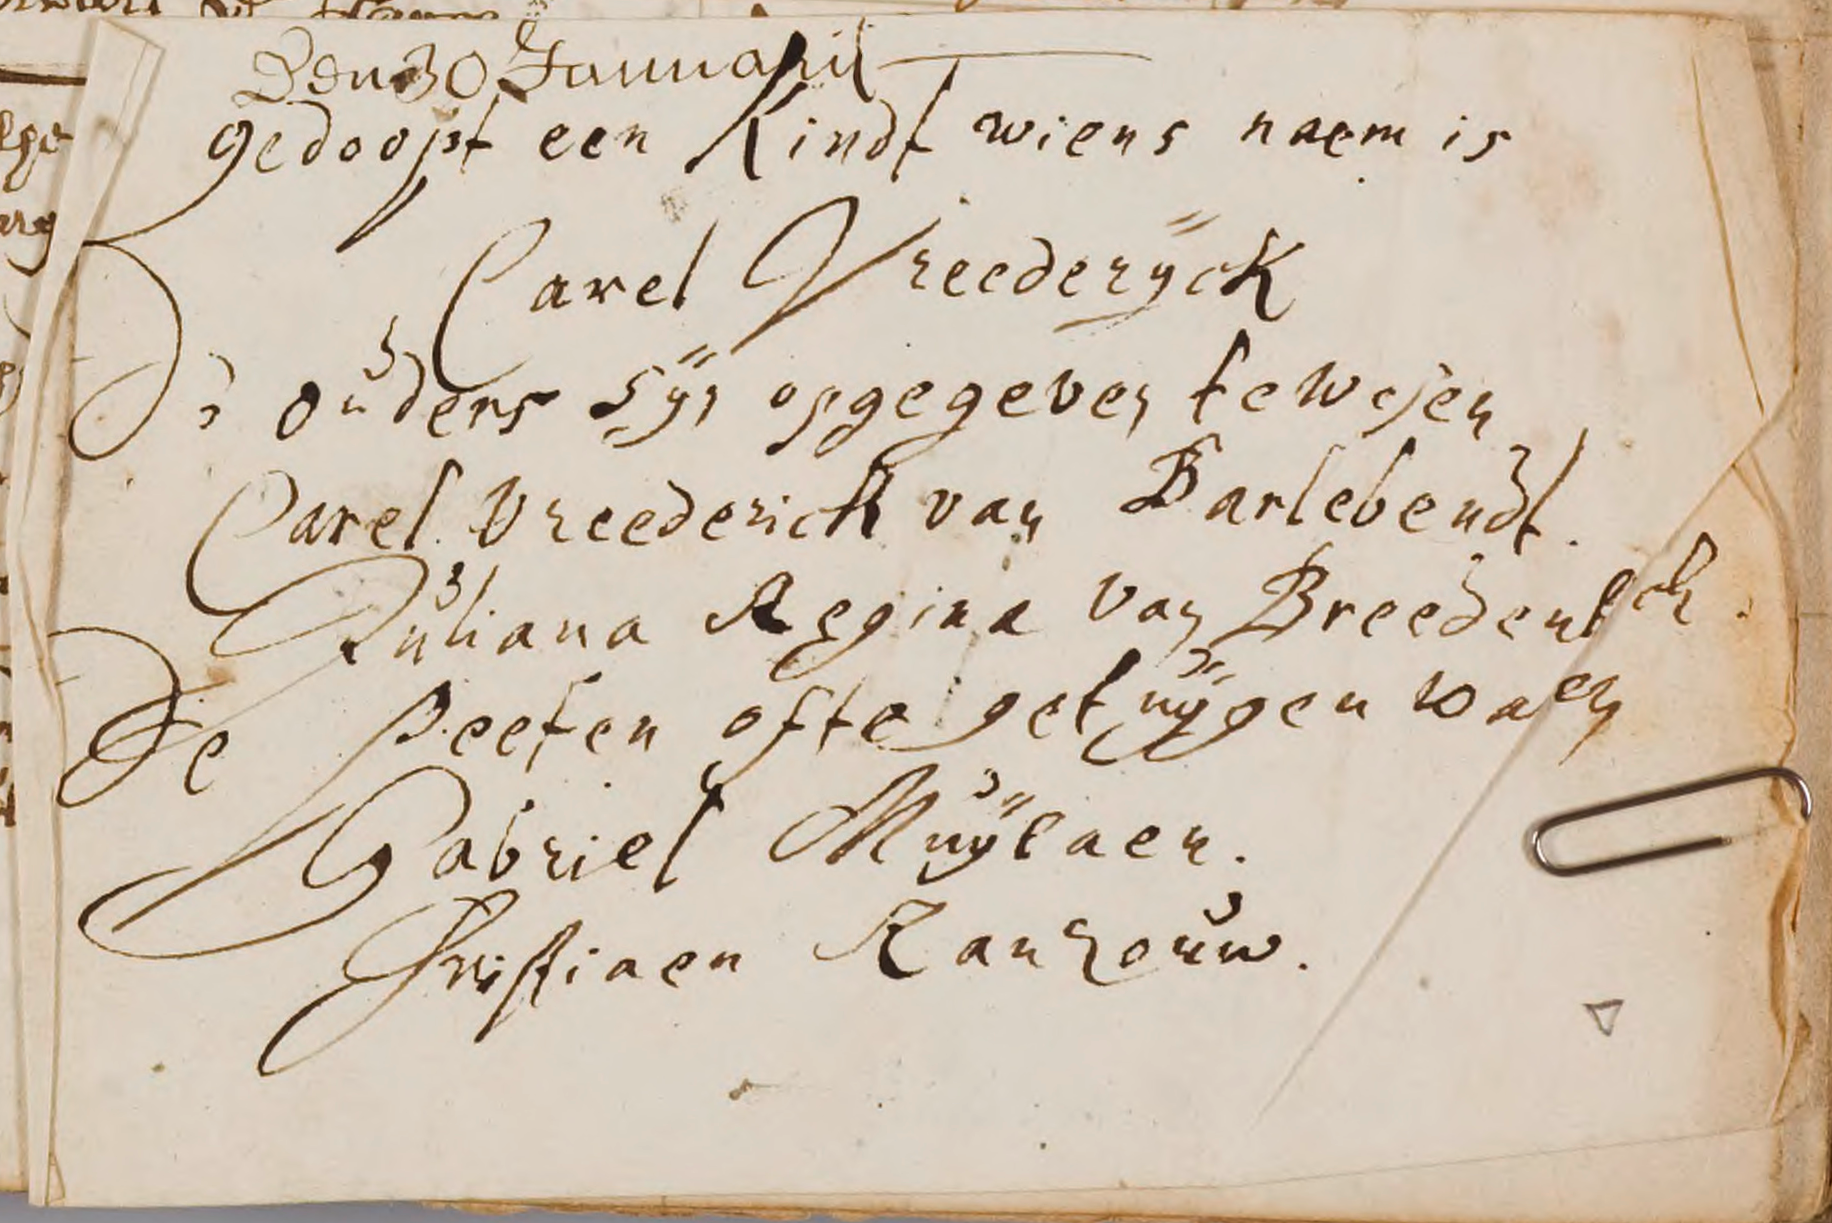
\includegraphics[width=\textwidth]{seddel.png}\\%
	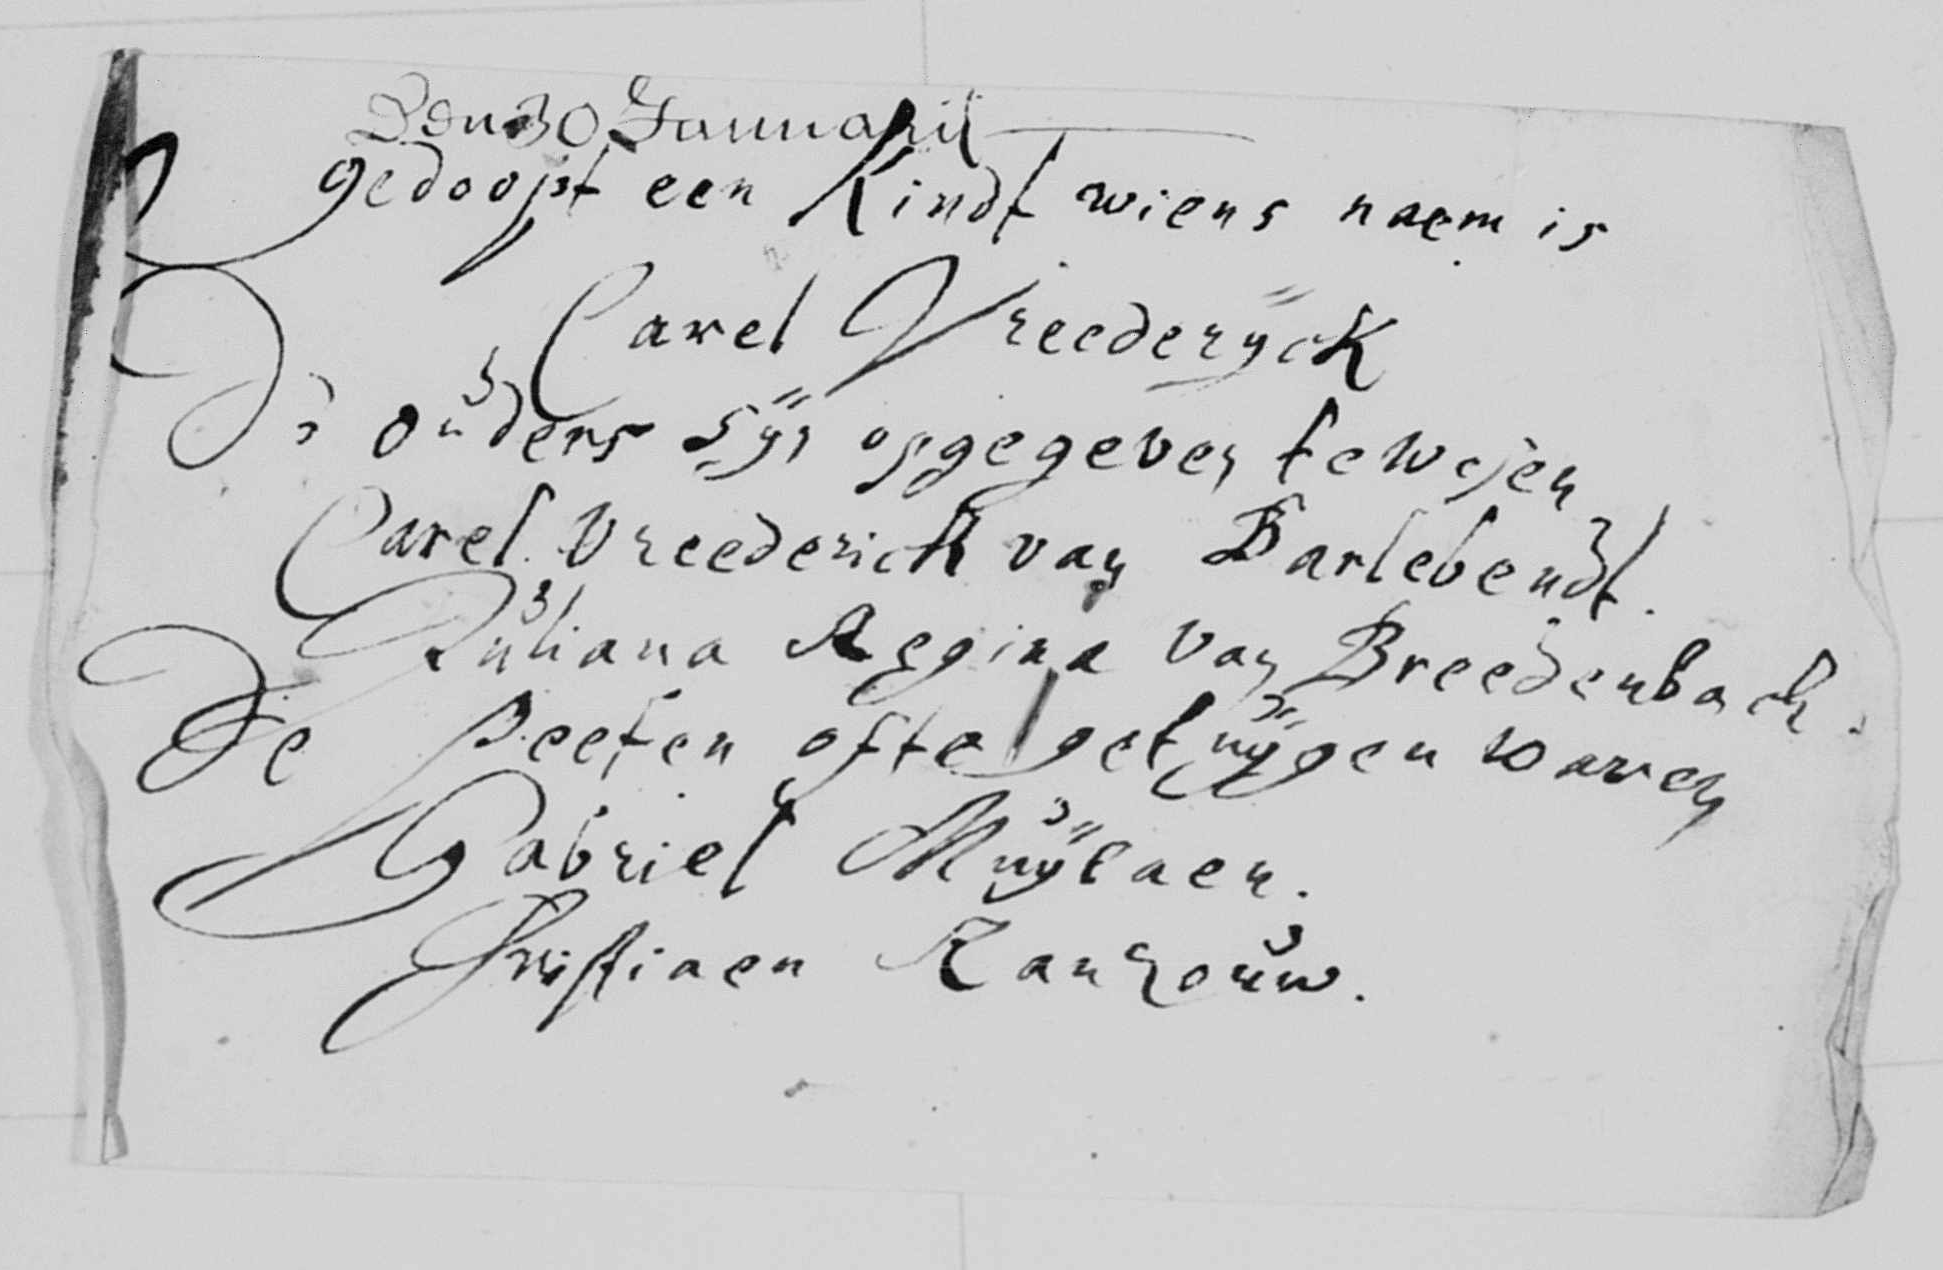
\includegraphics[width=\textwidth]{kb-old.png}\\%
	\caption{Digitaliseringer\\\smaller Øverst: Amsterdams Stadsarkivs affotografering fra 2010erne\\Nederst: FamilySearch's digitaliserede mikrofilm fra april 1950}%
\end{figure}%

\subsection{Videre Søgning}

\dropcap{D}{et maa formodes,} at ovennævnte Carel Vreederick van Barlebendt senior er afdød kort efter dåben, og at Milan og von Breitenbach er blevet viet kort efter. Den yngre van Barlebendt har derefter fået eller taget navnet Milan efter sin stedfader.

Hvis fadderen Christiaen Ranzouw er lig med Christian von Rantzau til Salzau, Rastorf og Bürau (20. aug 1649 Rastorf -- 17. aug 1704 Kiel), er det en mulighed at dåben reelt er foretaget i eller nær dennes hjemstavn. Rantzau ægteviet 1676 i Ascheberg, Slesvig-Holsten, imedens han boede på godset Salzau. Rantzau skal endvidere have været klosterprovst i Preetz, Slesvig-Holsten 1669--75, det har dog ikke været muligt at undersøge eventuelle kirkebøger derfra på skrivende fod.
% https://finnholbek.dk/getperson.php?personID=I649&tree=2

En anden mulighed er at det ikke er Carl Friderich Milans dåb der refereres på sedlen, men at han blev født senere og opkaldt efter sedlens hovedperson. Han kan så være døbt i Utrecht, jfr. brevet af 4. februar 1678 på \cpageref{brev1678}. Rigsbaron Jacob de Petersen fik en søn i Utrecht 1674, og hans hustru skal være død samme sted 1678; han skal desuden have ejet en lystgård i landsbyen 's-Graveland\footnote{Fr. Krarup, \emph{op.cit.}, s. 116}.
% https://biografiskleksikon.lex.dk/Jacob_Petersen

Følgende kirkebøger i Utrecht og 's-Graveland er undersøgt uden held:

\begin{description}[format=\normalfont, noitemsep]
\item[Utrecht, \emph{Alle gezindten\footnote{Hollandsk: \enquote{Alle menigheder}}, dopen 1675--79}]
	{\smaller\url{https://familysearch.org/pal:/MM9.3.1/TH-1942-33026-16505-17}}
\item[Utrecht, \emph{Nederlands Hervormd}, \emph{dopen 1665--92}]
	{\smaller\url{https://familysearch.org/pal:/MM9.3.1/TH-1951-33027-15097-74}}
\item[Utrecht, \emph{Doopsgezinde}, \emph{index geboorten 1659--80}]
	{\smaller\url{https://familysearch.org/pal:/MM9.3.1/TH-1971-28101-12220-85}}
\item[Utrecht, \emph{Remonstrant}, \emph{index dopen 1642--82}]
	{\smaller\url{https://familysearch.org/pal:/MM9.3.1/TH-1961-33031-25635-17}}
\item[Utrecht, \emph{Evangelisch Luthers}, \emph{dopen 1626--99}]
	{\smaller\url{https://familysearch.org/pal:/MM9.3.1/TH-1971-33038-1548-7}}
\item[Utrecht, \emph{Oud Katholiek}, \emph{dopen 1665--1810}]
	{\smaller\url{https://familysearch.org/pal:/MM9.3.1/TH-1951-33033-9102-51}}
\item[Utrecht, \emph{Rooms Katholiek}, \emph{dopen 1669--1811}]
	{\smaller\url{https://familysearch.org/pal:/MM9.3.1/TH-1942-33023-17697-63}}
\item['s-Graveland, \emph{Nederlands Hervormd}, \emph{dopen, trouwen 1658--1725}]
	{\smaller\url{https://familysearch.org/pal:/MM9.3.1/TH-1961-31188-9415-59}}
\end{description}

Det har desværre endnu ikke været muligt at finde noget videre om Carel Vreederick van Barlebendt senior, men der skal findes flere tyske adelsslægter \emph{Bardeleben}, hvor varianten \emph{Barleben} kendes i Magdeburg og Estland\footnote{  \url{https://de.wikipedia.org/wiki/Bardeleben_(Adelsgeschlechter)}}.

\section{Konkluſion}

\dropcap{M}{ed ovenſtaaende} in mente ser hypotesens kronologi således ud:

\begin{savenotes}%
\begin{figure}[H]%
\centerfloat%
\begin{tabular}{r p{.75\textwidth}}
	senest 1675 & Gabriel Milans første kone ... da Castro, datter af Benjamin Musaphia, død. Ministerialbøgerne fra \emph{Portugees-Israëlitisch Kerkgenootschap} i Amsterdam er undersøgt, men der er desværre en lakune i perioden ca. 1650--80 (ca. 5410--40 i den jødiske kalender). \\
	30. januar 1676 & Carel Vrederijck van Barlebendt junior døbt. Han bliver senere i livet kaldt Milan efter sin stedfar. \\
	--- & Carel Vrederijck van Barlebendt senior død, formentlig i Holland. \\
	--- & Gabriel Milan + Juliana Regina von Breitenbach viet, formentlig i Holland. \\
	juli 1678 & Gabriel Milan forlader Holland med Juliana Regina von Breitenbach og deres fælles børn samt stedbørn. \\
\end{tabular}%
\end{figure}%
\end{savenotes}

En endelig af- eller bekræftelse af hypotesen må søges ved at finde dokumentation for ovenstående begivenheder, i særdeleshed den ældre van Barlebendts død og vielsen mellem Milan og von Breitenbach. Amsterdams kirkebøger og \emph{Huwelijksaangiften} (notifikationer om intention om ægteskab) er undersøgt uden held, så (en del af) begivenhederne skal nok findes andetsteds, hvis kilderne er bevarede.

Sluttelig kan det siges, at eftersom hele Gabriel Milans kendte efterslægt nedstammer igennem Carl Friderich Milan og dennes afkom, er der --- hvis hypotesen holder --- ingen (kendte) nulevende efterkommere af Gabriel Milan.

\signatur{Mikkel Eide Eriksen\\
Nørrebro, 2014\\
Ajourført \the\year}%

\end{document}
